\documentclass[a4paper, 12pt]{report}
% Importation des paquets
\usepackage{graphicx} % Required for inserting images
\usepackage{wrapfig}
\usepackage[french]{babel}
\usepackage[T1]{fontenc} 
\usepackage{svg}    % Paquet pour afficher des SVG
\usepackage{minted} % Paquet pour la coloration syntaxique améliorée
\usepackage{blindtext}
\usepackage{titlesec}
\usepackage{hyperref}
\usepackage{multirow}
\usepackage{tabularx}
\usepackage{ltablex}
\usepackage{longtable}
\usepackage{biblatex}
\usepackage{csquotes}
\usepackage{listings}
\usepackage{float}

\lstset{language=Python} % Langage utilisé pour les listings

\addbibresource{Bibliographie.bib}

\usepackage[left=2cm, right=2cm, top=2cm, bottom=2cm]{geometry} % choix personnel de marges

% Variables d'environnement
\graphicspath{ {./Images/} }    % Chemin du dossier contenant les images

\usepackage{changepage}
\strictpagecheck

% Document

\title{M8}

\author{Alix ANNERAUD - Myriem ABID - Amandine BURCON}


\titleformat{\chapter}[display]{\normalfont\huge\bfseries}{}{0pt}{\Huge} % Formatage des chapitres

\newcommand{\pythoninline}[1]{\mintinline{python}{#1}}

\begin{document}

\begin{titlepage}
	\centering
	{\textsc{INSA Rouen Normandie} \par}
	\vspace{1cm}
	{\Large \textsc{Projet de M8}\par}
	\vspace{1.5cm}
	{\huge\bfseries Analyse de la dansabilité d'une musique\par}
	\vspace{2cm}
	{\Large\itshape Alix ANNERAUD - Myriem ABID - Amandine BURCON\par}
	\vfill
	supervisé par\par
	   M. GAUZERE

	\vfill

% Bottom of the page
	{\large \today\par}
\end{titlepage}



\tableofcontents

\chapter{Introduction}

\section{Motivation}

Quel est le lien entre l'analyse de données et une soirée réussie ? Cette question peut, de prime abord, paraître saugrenue...et pourtant !
Réponse : la sélection musicale idéale qui fera vibrer la piste de danse...

En effet, créer manuellement la playlist qui conviendra à une soirée peut rapidement s'avérer fastidieux et chronophage. C'est ici qu'entre en jeu la science des données qui permet de traiter, d'analyser et d'organiser de façon pertinente un volume important de données.

Nous organisons des soirées étudiantes et il nous a semblé judicieux de mettre à profit ce que nous avons appris en cours d'analyse de données pour déterminer quelles sont les chansons et musiques susceptibles de convenir au plus grand nombre et d'attirer les danseurs sur la piste de danse.

Notre objectif est d'utiliser les techniques de traitement des données vues en cours pour analyser une multitude de caractéristiques musicales. Nous examinerons des éléments tels que le tempo, la structure rythmique, l'énergie entre autres. En comprenant les facteurs qui contribuent à rendre une musique entraînante, nous pourrons créer des playlists qui garantiront une ambiance festive.

Le modèle développé permettra alors de déterminer la dansabilité d'une musique ce qui permet non seulement un gain de temps mais également d'optimiser la sélection effectuée grâce à la prise en compte de nombreux paramètres. Notre projet montre que l'analyse des données est un outil d'aide à la décision précieux et que les domaines d'application sont divers et variés.

\section{Organisation}

Pour notre projet, nous avons utilisé des outils permettant d'optimiser la collaboration entre les membres du groupe :
\begin{itemize}
    \item  \underline{GitHub :} Une plate-forme en ligne permettant d'héberger un répertoire Git.
    \item \underline{OverLeaf :} Une plate-forme en ligne permettant d'éditer en collaboration un document latex.
    \item \underline{Visual Studio Code :} Un éditeur de code très flexible.
    \item \underline{Jupyter extension for VSCode :} Une extension VSCode permettant une intégration de Jupyter.
    \item \underline{Live Share :} Une extension VSCode permettant de travailler en simultané sur le même code.
\end{itemize}

Notre répertoire de code se trouve à l'adresse suivante : \url{https://github.com/AlixANNERAUD/Projet-M8}.


\chapter{Description des données}

Le jeu de données\cite{Jeu_De_Donnees} comprend 19 caractéristiques (variables) de 169909 musiques (observations), sorties entre 1921 et 2020, dont certaines proviennent des top-100 de chaque années. Ce dernier a lui même été extrait à partir de l'API Web de Spotify\cite{Spotify_for_Developers_API}, que nous allons nous aussi utiliser à la fin de ce projet pour mettre en pratique notre modèle.

Les variables de notre jeu de données et leurs caractéristiques sont les suivantes: 

\begin{longtable}{|p{0.25\linewidth}|p{0.20\linewidth}|p{0.45\linewidth}|}
\hline
\textbf{Nom} & \textbf{Type} & \textbf{Description} \\
\hline
\verb|acousticness| & Quantitative continue & De 0,0 à 1,0, permet de déterminer si la piste est acoustique. 1,0 représente une probabilité élevée que la piste soit acoustique. \\
\hline
\verb|artists| & Qualitative & Tableau de chaînes de caractères contenant tous les artistes. \\
\hline
\verb|dansability| & Quantitative continue & Décrit dans quelle mesure un morceau se prête à la danse. De 0,0 à 1,0 en dansabilité croissante. \\
\hline
\verb|duration_ms| & Quantitative discrète & La durée de la piste en millisecondes. \\
\hline
\verb|energy| & Quantitative continue & De 0,0 à 1,0, représente une mesure perceptuelle de l'intensité. En règle générale, les morceaux énergiques sont rapides, forts et bruyants. Les caractéristiques y contribuant comprennent la gamme dynamique, l'intensité sonore perçue, le timbre, la vitesse d'apparition et l'entropie générale. \\
\hline
\verb|explicit| & Qualitative & Indique si la musique est explicite (destinée à un public adulte) ou non. \\
\hline
\verb|id| & Chaîne de caractères & Identifiant Spotify de la musique. \\
\hline
\verb|instrumentalness| & Quantitative continue & Détermine si une piste est majoritairement musicale. Les vocalises sont considérées comme instrumentales. Plus la valeur est proche de 1,0, plus la piste est exclusivement musicale. \\
\hline
\verb|key| & Qualitative & Entier représentant la tonalité de la piste. Les nombres correspondent aux hauteurs en utilisant la notation standard de la classe de hauteur. Si aucune clé n'a été détectée, la valeur est -1. \\
\hline
\verb|liveness| & Quantitative continue & Détecte la présence d'un public dans l'enregistrement. Des valeurs plus élevées représentent une probabilité accrue que la piste ait été jouée en direct, avec une quasi certitude au-dessus de 0.8. \\
\hline
\verb|loudness| & Quantitative continue & L'intensité sonore globale d'une piste en décibels (dB), calculée en moyenne sur l'ensemble de la piste. Les valeurs se situent généralement entre -60 et 0 dB. \\
\hline
\verb|mode| & Qualitative & Indique la modulation (majeure ou mineure) d'une piste. \\
\hline
\verb|name| & Chaîne de caractères & Nom du titre. \\
\hline
\verb|popularity| & Quantitative discrète & La popularité d'une musique \\
\hline
\verb|release_date| & Chaîne de caractères & Date de sortie de la musique au format AAAA-MM-JJ. \\
\hline
\verb|speechiness| & Quantitative continue & Représente la présence de mots parlés dans une piste. Les valeurs supérieures à 0,66 décrivent des pistes probablement composées exclusivement de paroles. Entre 0,33 et 0,66, les pistes peuvent contenir à la fois de la musique et de la parole, soit en sections, soit en couches. Les valeurs inférieures à 0,33 représentent très probablement de la musique. \\
\hline
\verb|tempo| & Quantitative discrète & Le tempo global estimé d'une piste en battements par minute (BPM). \\
\hline
\verb|valence| & Quantitative continue & Entre 0,0 et 1,0, décrit la positivité musicale transmise par une piste. Les morceaux ayant une valence élevée sonnent plus positivement. \\
\hline
\verb|year| & Quantitative discrète & Année de sortie. \\
\hline
\caption{Tableau des différentes variables du jeu de donnée.}
\end{longtable}

Des 19 caractéristiques disponibles pour l'analyse, nous allons ignorer quatre variables : \verb|id|, \verb|name| et \verb|artists| qui n'ont pas d'intérêt particulier, et \verb|release_date|, car elle est redondante avec la variable \verb|year|. 

\section{Représentation graphique}

Afin de mieux comprendre notre jeu de données et de pouvoir par la suite interpréter nos résultats, nous avons représenté graphiquement quelques-unes des variables dont nous disposions.

\subsection{Variables qualitatives}

\subsubsection{Artistes}

Comme une musique comprend plusieurs artistes, et que ces derniers sont stockés dans des tableaux, nous n'avons pas pu utiliser la méthode \pythoninline{np.unique(...)} pour déterminer les modalités ainsi que la fréquence de la variable \verb|artists|. A la place, nous avons eu recourt à un "dictionnaire" python, dans lequel les artistes sont ajoutés et leur fréquence incrémentée en fonction de leur présence dans le dictionnaire. Nous avons présenté nos résultats dans le diagramme en barre ci-dessous. On peut remarquer que la plupart sont des compositeurs de musique classique.

 \begin{figure}[h]
     \centering
     \includesvg[width=0.75\linewidth]{Artistes les plus fréquents.svg}
     \caption{10 Artistes les plus fréquents}
 \end{figure}

\subsubsection{Explicite}
\begin{figure}[!h]
    \centering
\includesvg[width=0.75\linewidth]{Images/Répartition des musiques destinées à un public averti.svg}
    \caption{Proportion de données explicites}
\end{figure} 


Les plateformes de streaming précisent généralement si une musique est explicite ou non, c'est une mention qui permet d'indiquer si une musique a un contenu offensant ou inapproprié pour les mineurs. Cela nous semblait pertinent de se faire une idée de la part de musiques explicites présentes dans notre jeu de données. Nous avons donc comptabilisé le nombre de fois qu'apparaît chaque modalité de la variable "explicit" (True et False). 


On peut conclure que la majorité des musiques étudiées ne sont pas explicites, il faudra donc potentiellement prendre en compte la différence de taille des échantillons si on les compare.


\subsubsection{Tonalités}

Chaque musique dispose d'une tonalité (variable \verb|key|). Nous avons étudié la répartition des tonalités à l'aide d'une pie chart et avons fait quelques observations: la tonalité Ré\# possède un pourcentage inférieur à 5\%, Fa\# a un pourcentage de 5.1\%. Hormis ces valeurs, il n'y a pas de gros écarts entre les distributions des différentes tonalités, tous les pourcentages sont entre 6\% et 12\%.

\begin{figure}[!h]
    \centering
    \includesvg[width=0.75\linewidth]{Images/Répartition de la tonalité des musiques.svg}
    \caption{Proportions des tonalités}
\end{figure}

\subsection{Variables quantitatives discrètes}

\subsubsection{Année}

Nous nous sommes également intéressés à la répartition des musiques par année. Pour ce faire, nous avons comptabilisé le nombre d'apparition de chaque année dans notre jeu de données. On constate que les années sont représentées de manière uniforme à partir de 1950, avec 2000 musiques par année. Cela montre qu'il y a une répartition uniforme au sein du jeu de données, ce qui est nécessaire pour avoir la représentation la plus objective possible. Cependant, on constate tout de même un manque de musiques avant 1950, dû au fait que les musiques de cette époque ne sont pas assez représentées dans les plateformes de streaming. Ce manque de représentation peut être expliqué par la présence de contrats de licence entre les maisons de disque et les plateformes de streaming, la différence des méthodes d'enregistrement d'époque et le coût que cela peut engendrer de les numériser, ou encore les nombreuses périodes de crise qui ont eu lieu entre 1920 et 1950 (Grande Dépression, Seconde Guerre Mondiale...).

\begin{figure}[!h]
    \centering
\includesvg[width=0.75\linewidth]{Images/Répartition des musiques par année.svg}
    \caption{Répartition temporelle des données}
\end{figure}

\subsection{Variables quantitatives continues}



\begin{figure}[htbp]
    \begin{minipage}[t]{0.49\textwidth}
        \centering
        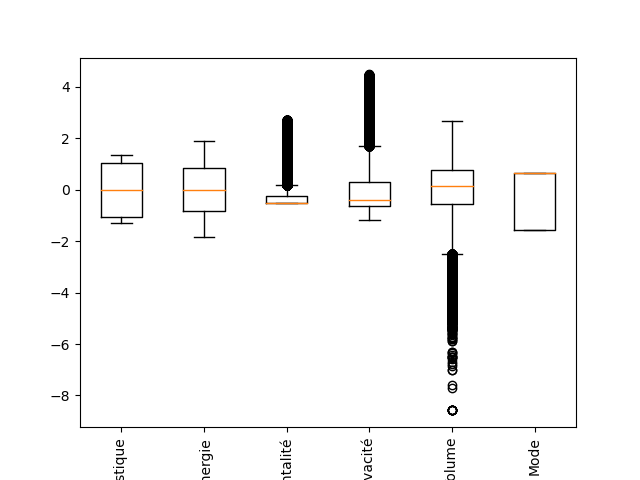
\includegraphics[width=\textwidth]{Images/Boîte à moustache des variables 1 à 6.png}
    \end{minipage}\hfill
    \begin{minipage}[t]{0.49\textwidth}
        \centering
        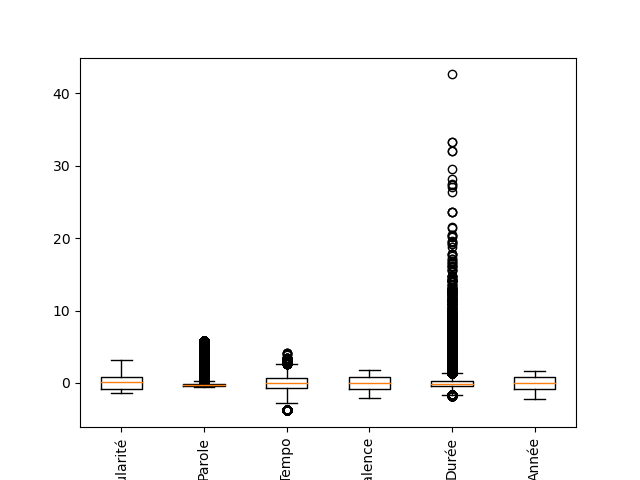
\includegraphics[width=\textwidth]{Images/Boîte à moustache des variables 7 à 12.png}
    \end{minipage}
    
    \caption{Représentation des variables continues normalisées}
    \label{fig:enter-label}
\end{figure}

Les variables quantitatives peuvent être toutes représentées sur un même graphe, ce qui nous permet de les visualiser plus facilement. Elles ont également été normalisées afin d'avoir des échelles comparables.



On remarque un nombre important de valeurs extrêmes pour plusieurs variables, ce qu'on peut comprendre au vu de la diversité de nos données. Les pistes ayant une instrumentalité, une vivacité ou une durée élevée, ou encore un volume très bas sont nombreuses mais restent une minorité face au reste des morceaux.

\section{Préparation des données}

\subsection{Conversions}

Notre objectif étant de réaliser un modèle de régression linéaire, il nous faut alors impérativement des variables quantitatives continues.

Tout d'abord, nous avons intégré les variables quantitatives continues dans la matrice sur laquelle nous allons travailler plus tard.

Ensuite, concernant les variables quantitatives discrètes, nous avons jugé qu'elles pouvaient toutes être interprétées comme des variables quantitatives continues car elles comportent un nombre limité de valeurs ordinales.

Enfin, concernant les variables qualitatives qui présentaient un certain intérêt pour l'analyse (\verb|key|), nous avons effectué une conversion avec la méthode de l'encodage 1 parmi n (alias encodage "one-hot"), qui consiste simplement à convertir les modalités d'une variable qualitative en plusieurs variables booléennes, que l'on peut considérer ensuite comme quantitatives.\cite{Encodage_1_parmis_n}

Cette approche possède cependant quelques restrictions : 
\begin{itemize}
    \item Il faut que la variable possède un nombre fini de modalités.
\end{itemize}

Cette approche à été utilisée pour la variable \verb|key|.

\subsection{Classe}

Par soucis de concision et de lisibilité du code, nous avons implémenté une classe qui permettra d'en-capsuler nos matrices de données. Son fonctionnement est simple: lorsque le constructeur de la classe est appelé, la matrice donnée est d'abord copiée dans un attribut de la classe, puis une version normalisée est également stockée en tant qu'attribut (si nécessaire). Cela évite ainsi d'avoir à utiliser de multiples variables (matrice, matrice normalisée, moyenne, nombre de variables etc.).

Le constructeur de cette dernière prend pour argument :
\begin{itemize}
    \item \pythoninline{X} (\pythoninline{numpy.ndarray}) : La matrice à en-capsuler.
    \item \pythoninline{Labels}  (\pythoninline{list}): Les étiquettes des variables de la matrice.
    \item \pythoninline{Already_Scaled}  (\pythoninline{bool}) : Détermine si les données doivent être normalisées ou non (\pythoninline{True} par défaut).
\end{itemize}

Cette dernière contient les méthodes suivantes :
\begin{itemize}
    \item \pythoninline{Raw()} : Retourne la matrice brute (non normalisée).
    \item \pythoninline{Scaled()} : Retourne la version normalisée de la matrice.
    \item \pythoninline{Variables()} : Retourne le nombre de variables décrites par la matrice.
    \item \pythoninline{Observations()} : Retourne le nombre d'observations contenues par la matrice.
    \item \pythoninline{Mean()} : Retourne les moyennes des différentes variables de la matrice brute.
    \item \pythoninline{Standard_Deviation()} : Retourne l'écart-type des différentes variables de la matrice brute.
    \item \pythoninline{Labels()} : Retourne les étiquettes des variables de la matrice.
\end{itemize}


\chapter{Analyse}

\section{Analyse en composantes principales}

Dans une tentative de simplifier nos analyses et de mieux visualiser nos données, nous avons fait le choix de réaliser une analyse en composantes principales. On commence alors par calculer la matrice de corrélation, point de départ de cette analyse. 
\begin{figure} [h]
    \centering
    \includesvg{Matrice de corrélation.svg}
    \caption{Matrice de corrélation}
    \label{fig:enter-label}
\end{figure}

Nous avons bien une matrice de corrélation dont les valeurs de la diagonale dominante sont égales à 1 ce qui est logique étant donné qu'elles représentent la corrélation d'une variable avec elle-même. On remarque également que certaines variables semblent liées:

\begin{itemize}
    \item \verb|acousticness| avec \verb|energy|, \verb|popularity| et \verb|year| : il semblerait que plus une musique est acoustique, moins elle est énergique, populaire et récente.
    \item \verb|volume| et \verb|year|. Il semblerait qu'une musique est plus énergique si le volume est plus haut.
    \item \verb|popularity| avec \verb|year|. Il semblerait que plus une musique est récente, plus elle est populaire.
\end{itemize}

La matrice de corrélation étant aux normes, nous pouvons appliquer l'ACP. Nous affichons le pourcentage de variance expliqué par chaque axe ainsi que le pourcentage cumulé de variance expliqué. 

\begin{figure} [h]
    \centering
    \includesvg[width=0.75\linewidth]{Images/Pourcentage de variance expliquée par les composantes principales.svg}
    \caption{Variance expliquée par les composantes principales}
    \label{fig:enter-label}
\end{figure}

Les résultats ne sont pas très concluants. En effet, la variance semble être expliquée par quasiment chaque variable. Il nous faudrait 16 variables sur les 24 étudiées pour expliquer 80\% de la variance. Nous en déduisons que l'intérêt de l'ACP dans notre cas est assez limité car elle ne nous a pas réellement permis de distinguer un sous-ensemble de composantes principales dominantes qui permettrait d'expliquer une grande partie de la variance de nos données.


\section{Régression linéaire}

Afin de savoir si une musique est dansable à partir de ses données, il nous faut un modèle de prédiction. Nous avons donc utilisé une régression linéaire multiple pour créer notre modèle et effectuer nos prédictions. Il est important de noter que, comme nos données se basent sur le calcul de la dansabilité de Spotify, notre modèle va ainsi tenter de reproduire le fonctionnement de ce dernier à partir des données dont nous disposons. Nous verrons à l'issue de la régression linéaire multiple si le modèle en ressortant serait satisfaisant. 

On définit pour cela une fonction qui déterminera la solution du système ainsi que d'autres indicateurs. Nous utiliserons les formules suivantes: 
\begin{itemize}
    \item Système : $\hat{y} = \beta_0 + \beta_1 x_1 + \beta_2 x_2 + ... + \beta_n x_n$.
    \item Résidus : $e_i = y_i - \hat{y_i}$.
    \item Coefficient de détermination : $R^2 = 1 - \frac{\sum_{i=1}^{n} (y_i - \hat{y_i})^2}{\sum_{i=1}^{n} (y_i - \bar{y})^2}$.
    \item Estimation non biaisée de la variance : $\hat{\sigma}^2 = \frac{\sum_{i=1}^{n} e_i^2}{n-p-1}$. 
\end{itemize}

Afin de visualiser nos résultats, nous avons affiché les nuages de points correspondants à notre régression linéaire, ils sont disponibles dans le notebook du projet. Nous affichons également les coefficients de la régression linéaire multiple, pour visualiser plus facilement l'importance de chaque variable:

\begin{figure} [h]
    \centering
    \includesvg[width=0.75\linewidth]{Images/Régression linéaire de la dansabilité en fonction des caractéristiques continues.svg}
    \caption{Coefficients de la régression linéaire par variable continue}
    \label{fig:enter-label}
\end{figure}


On se rend alors compte que les variables favorisant le plus la dansabilité d'une musique sont : \verb|valence|, \verb|speechiness|, \verb|year| et \verb|popularity|.

On pourrait penser que la tonalité d'une musique n'a pas d'effet sur sa dansabilité, mais on remarque que les musiques en Do\# sont les plus dansables. C'est bien cohérent avec les résultats de l'ACP.

D'un autre côté, les variables qui défavorisent le plus la dansabilité d'une musique sont : \verb|acousticness|, \verb|energy| et \verb|liveness|.

Les autres variables ne semblent pas contribuer de manière significative à la dansabilité d'une musique.

Ces résultats sont cohérents avec les résultats de l'ACP, mais également avec le sens commun. Le seul résultat étrange est l'effet négatif de l'énergie de la musique, mais nous ne connaissons pas la manière dont elle est mesurée. La subjectivité de cette variable est une explication possible à ce résultat.

Cependant, bien que ces résultats nous paraissent cohérents (subjectivement), le coefficient de détermination $R^2$ de notre modèle est bien trop bas pour que notre régression soit considérée comme satisfaisante. Parmi les raisons qui peuvent nuire à notre régression, nous avons : 

\begin{itemize}
    \item  \underline{Mauvais modèle :} En effet, nous avons utilisé un modèle de régression linéaire. Cependant, il se pourrait que Spotify ait utilisé un modèle de régression polynomial, voire un modèle tout autre et plus complexe qu'un modèle de régression.
    \item \underline{Variables manquantes :} Notre jeu de données, bien qu'il comprend beaucoup de variables et d'observations, n'est peut être pas assez complet. En effet, il se pourrait que Spotify se base sur d'autres variables, qui ne sont pas disponibles dans ce jeu de données.
    \item \underline{Variables inappropriées :} A contrario de l'hypothèse précédente, il se pourrait également que certaines de nos variables nuisent à la qualité de notre régression. En effet, nous avons utilisé toutes les variables à notre disposition. Cependant, peut être que certaines ne sont pas pertinentes pour notre analyse.
    \item \underline{Observations erronées :} Bien que les valeurs du jeu de données se basent sur des calculs et analyses mathématiques faites par Spotify au préalable, il est possible que certaines musiques soient des cas particuliers (par exemple : live de concerts, ...).
\end{itemize}

\section{Diagnostic}

Comme expliqué précédemment, la qualité de notre régression linéaire multiple n'était pas très bonne. Cela était prévisible au vu de la quantité et du nombre de variables qui ont été utilisées. Ainsi, afin d'y remédier, nous avons procédé à un nettoyage de nos données.

\subsection{Sélection de variables}

Tout d'abord, nous commençons notre nettoyage par éliminer des variables qui nuisent à la précision de notre jeu de données. Pour cela nous avons utilisé le \(C_p\) de Mallows, calculé par la fonction \pythoninline{Get_Cp_Mallows()}. Les \(C_p\) de Mallows sont alors calculés pour chaque combinaison possible de variables. Ces calculs sont fait par sélection ascendante avec la fonction  \pythoninline{Forward_Selection()} où chaque variable est ajoutée une a une. Une fois toutes les combinaisons calculées, le modèle retenu est celui possédant le \(C_p\) de Mallows le plus bas. La fonction renvoie alors les variables sélectionnées, en plus du coefficient de détermination et du \(C_p\) du modèle correspondant. 

Ainsi, notre jeu de données passe de 24 à 20 variables, les variables qui sont éliminées étant toutes des clés : \verb|Do|, \verb|Fa#|, \verb|Sol#| et \verb|La#|.

\subsection{Élimination des valeurs aberrantes}

Bien que le jeu de données que nous avons ne comporte pas d'erreurs de mesures, il est tout de même essentiel d'éliminer certaines valeurs. En effet, la majorité de notre jeu de données est constitué de musiques et chansons, mais il contient également quelques podcasts, ou versions en présence de public par exemple, que nous ne voulons pas prendre en compte car cela donne lieu à des valeurs extrêmes qui perturbent notre modèle.

Pour cela, nous utilisons comme indicateur la contribution de chaque valeur à la régression linéaire.

Afin d'obtenir la contribution, nous effectuons le calcul des leviers avec la formule : \(H = X (X^\top X)^{-1}X^\top\), la valeur des leviers pour chaque observation se situant sur la diagonale de la matrice \(H\). Une fois les leviers obtenus, on procède  au calcul des contributions avec cette formule : \(c_i = \frac{H_{ii}}{(1 - H_{ii})^2}\frac{\hat \varepsilon_i^2}{p s^2}\). Ces calculs sont effectués par la fonction \pythoninline{Linear_Regression_Metrics()}. Cependant, notre jeu de données étant trop conséquent, il a fallu procéder par "blocs", en effectuant des régressions linéaires pour chaque bloc de données (\pythoninline{Line_Regression_Metrics_Blocks()}).

Une fois le calcul des contributions effectué, nous avons procédé à la phase d'élimination. Ainsi, on va définir un seuil de contribution limite. Une observation possédant ainsi une contribution au delà de ce seuil se verra alors éliminé du jeu de données. Une fois notre jeu de données nettoyé de ces valeurs aberrantes, nous avons créé un nouveau modèle de régression linéaire, et nous avons constaté une amélioration du coefficient de détermination comme attendu.

Il nous faut cependant retirer une très grande quantité de données pour obtenir un $R^2$ réellement satisfaisant, la dansabilité n'est donc pas influencée linéairement par les autres variables dans un cas général. On peut tout de même considérer ce modèle linéaire comme valide en gardant une partie des données, ce qui nous paraît suffisant pour notre projet. 

\section{Tests statistiques}

Afin d'avoir une meilleure compréhension de ce qui influence la dansabilité, nous avons voulu vérifier à l'aide de tests la dépendance de variables deux à deux. Finalement, d'autres variables de notre jeu de données nous ont semblées pouvoir avoir un lien, et nous avons décidé de tester l'indépendance de la variable \verb|explicit| avec \verb|danceability| et \verb|popularity|.

\subsection{Normalité de la dansabilité}

En affichant la répartition de la dansabilité, il nous a semblé que cette variable avait l'air de correspondre à une loi normale. Nous avons donc décidé de vérifier notre hypothèse grâce au test de Shapiro-Wilk. Pour ce test, nous choisissons $\alpha = 0.05$ et l'hypothèse $H_0$ est que la dansabilité suit une loi normale. 

A l'aide de la fonction \pythoninline{scipy.stats.shapiro}, on trouve une p\_value de 9.4215e-07, ce qui est inférieur au seuil de 0.05 choisi. On rejette donc $H_0$, ce qui signifie que la variable \verb|danceability| ne suit pas une distribution normale.

Au vu de la taille de notre jeu de données, ce test a dû être réalisé sur seulement une subdivision  de nos données. Nous avons alors réalisé le test avec de plus en plus de valeurs et observé que la p-valeur diminue au fur et à mesure et tend vers 0.0, jusqu'à ce que la taille du vecteur de données testées soit trop importante pour réaliser le test. 

\subsection{Explicite et Dansabilité}

\begin{figure}[!h]
    \centering
    \includesvg[width=0.75\linewidth]{Images/Boîte à moustaches de la dansabilité des musiques explicites et non-explicites.svg}
    \caption{Dansabilité des musiques en fonction de la variable \textit{explicit}}
\end{figure}

Afin de savoir si le fait qu'une musique soit explicite ou non influence la dansabilité de cette dernière, nous avons commencé par afficher les boîtes à moustaches de la dansabilité des musiques explicites et celle des musiques non-explicites pour les comparer. 


On peut voir que la médiane de dansabilité des musiques explicites est plus élevée que celle des musiques non-explicites. Afin de vérifier si ce résultat indique que les musiques explicites sont plus dansables que les musiques non-explicites, nous effectuons un test de Student. Nous pouvons réaliser ce test car nous avons bien des échantillons indépendants et leurs tailles sont supérieures à 30. Nous choisissons un seuil $\alpha =0.05$ et formulons les hypothèses suivantes :

\begin{itemize}
    \item \(\mathcal{H_0}\) : Les musiques explicites ne sont pas plus dansables que les musiques non-explicites.
    \item \(\mathcal{H_1}\): Les musiques explicites sont plus dansables que les musiques non-explicites.
\end{itemize}

Après calcul, nous obtenons une p-valeur de 0.0. Cette valeur est inférieure à $\alpha$, ce qui signifie que $H_0$ est rejetée. On peut donc conclure que les musiques explicites sont les plus dansables. 

Cette valeur de $p = 0.0$ exacte semble être suspecte. En effet, il est impossible d'avoir une probabilité de se tromper complètement nulle. Cela nous pousse à douter de la fiabilité de nos résultats.

Cependant, il est important de noter que le test précédent a dû être réalisé sur seulement un nombre limité de données mais que sa p-valeur tendait vers 0.0 à l'ajout de données. Il est donc possible qu'ici p soit affiché égal à 0.0 exactement car la précision de la machine ne permet pas de donner sa valeur exacte. 

\subsection{Explicite et Popularité}

Cette fois-ci, nous nous intéressons aux variables \verb|explicit| et popularité (\verb|popularity|). Nous allons essayer de voir si le fait qu'une musique soit explicite impacte sa popularité. Nous procédons à nouveau à un test de Student dont les hypothèses sont :
\begin{itemize}
    \item \(H_0\) : Les musiques explicites ne sont pas plus populaires que les musiques non-explicites.
    \item \(H_1\) : Les musiques explicites sont plus populaires que les musiques non-explicites.
\end{itemize}
Les calculs effectués nous permettent d'obtenir une p-valeur de 2.0165324869979728e-05 ce qui est inférieur au seuil $\alpha = 0.05$ que nous avions fixé au début du test. Ce résultat nous permet de dire qu'il y a suffisamment de preuves pour rejeter l'hypothèse nulle, la différence entre les moyennes des deux catégories est donc significative. Cela va dans le sens de nos observations initiales. Une interprétation possible de ces résultats est que le rap et la hip-hop, qui ont tendance à être plus explicites que d'autres genres musicaux, ont gagné en popularité sur les plateformes de streaming. Cependant, cette interprétation ne reste qu'une hypothèse car nous ne pouvons pas la vérifier avec le jeu de données dont nous disposons étant donné que nous n'avons pas de variable spécifiant le genre musical des musiques présentes dans ce jeu de données.

\chapter{Application}

Une fois que notre modèle est correctement entraîné avec des données "propres", nous pouvons enfin passer à une application concrète, présentée en introduction. Ainsi, à partir du module python SpotiPy\cite{SpotiPy_Documentation}, nous avons pu utiliser l'API Spotify\cite{Spotify_for_Developers_API}.

\begin{enumerate}
    \item On récupère les résultats de recherche sur Spotify de notre musique.
    \item On sélectionne un des résultats, pour obtenir l'identifiant Spotify de la musique en question.
    \item On récupère les données correspondantes à la musique qui serviront au modèle pour sa prédiction. Puis on centre et on réduit ces données.
    \item On effectue une prédiction à partir du modèle.
    \item On récupère la dansabilité de la musique en question.
    \item On affiche les résultats.
\end{enumerate}

Les résultats que nous obtenons sont très proches des valeurs de dansabilité proposées par Spotify, on décide donc que notre modèle est satisfaisant.

\chapter{Difficultés}

\section{Taille du jeu de données}

Comme mentionné au début du rapport, le jeu de données que nous avons utilisé est assez volumineux : 19 variables pour 169909 observations. Normalement, cela ne pose aucun problème majeur pour la plupart des analyses, bien que cela puisse ralentir certaines opérations.

Cependant, certaines opérations telles que le produit d'une matrice par sa transposée (\(X^{T}\cdot X\)) pose un réel souci de complexité de mémoire. En effet, le produit d'une matrice de dimension \(n\times p\) par sa transposée donne une matrice de taille \(n\times n\).

Dans notre cas, lors du calcul des leviers en effectuant le produit de la matrice \pythoninline{X} pour le calcul du levier, nous nous retrouvions alors avec une matrice de \(169909\times169909\).

Or, sur un ordinateur récent (à taille de registre de 64-bits), où un nombre flottant est représenté par 8 octets, l'allocation mémoire nécessaire serait de : \(169909^{2}\times 8\simeq231\times10^{9}\) octets, soit 231 gigaoctets. Cependant, la taille moyenne de la mémoire RAM d'un ordinateur domestique est d'environ 8 gigaoctets.

Même si les systèmes d'exploitation modernes offrent un système de mémoire virtuelle permettant de stocker une partie de la mémoire sur le disque dur lorsque la RAM physique est insuffisante, cela reste une opération très coûteuse en termes de performances et nécessite un espace disque considérable.

Dans le cas où nous souhaitions calculer les leviers, nous avions besoin de faire un calcul d'une matrice par sa transposée : \(H = X (X^\top X)^{-1}X^\top\). Nous avons donc dû nous pencher sur une autre approche qui consiste à diviser notre jeu de données en blocs (dans l'axe des observations) et d'effectuer le calcul des leviers et contributions localement. Voici la démarche que nous avons suivi pour chaque bloc :

\begin{enumerate}
    \item On calcule les indexes de début et de fin du bloc à traiter.
    \item On extrait le bloc correspondant.
    \item On effectue une régression linéaire localement afin d'obtenir les résidus.
    \item On effectue le calcul des leviers et contribution pour le bloc.
    \item On sauvegarde les résultats obtenus dans l'emplacement correspondant des vecteurs de leviers et contributions.
\end{enumerate}

Dans le cas d'un bloc de 1000 observations, la taille maximale d'une matrice allouée était de \(1000^{2}\times 8 = 8 \times 10^{6}\) octets, soit 8 megaoctets, ce qui est raisonnable.

Les inconvénients de cette approche sont que les données ne sont peut être pas uniformément réparties dans le jeu de données, ce qui fait que le calcul des leviers et contribution peut être imprécis.

\chapter{Conclusion}

En conclusion, ce projet nous a permis d'appliquer les notions vues tout au long du semestre dans le cours de M8. Nous avons également pu l'étoffer en recherchant des compléments au cours. Cependant, nous étions tout de même limités par nos connaissances par moments. Il a été difficile d'innover pour proposer un projet avec une application intéressante à partir de ce jeu de données. 

Nous avons pu réfléchir de nous-mêmes aux différents jeux de données qu'il était possible d'étudier et quelle application nous pouvions tirer de leur analyse. Cela nous a également permis d'appréhender l'étude d'un jeu de données par nos propres moyens. Nous avons alors représenté quelques données graphiquement afin de décrire nos variables, nous nous sommes servis de l'ACP pour trouver des relations entre nos variables et nous avons réalisé une régression linéaire multiple pour obtenir un modèle utilisable dans notre application. Tout au long de ces étapes, nous étions dans une démarche de vérification de nos résultats, ce qui nous a poussé à réviser le modèle obtenu par la régression linéaire et à nettoyer les données utilisées. Nous avons également effectué des tests (Student, Shapiro-Wilk) dans le but de confirmer ou d'infirmer des hypothèses que nous avions formulées sur des couples de variables.

Bien que le modèle développé ne soit pas le plus performant et qu'il ne soit pas à destination d'une application réelle, nous considérons que nous avons réussi à atteindre l'objectif qui a motivé le sujet de ce projet compte tenu du fait que nous sommes débutants en matière d'analyse de données. Toutefois, il serait intéressant d'améliorer ce modèle en intégrant d'autres variables dans l'étude et en se penchant plus en détail sur la façon dont Spotify calcule réellement la dansabilité d'une musique.


\printbibliography[heading=bibintoc]


\end{document}
